\documentclass[pdftex,11pt]{article}
\usepackage[pdftex]{graphicx}
\usepackage{enumerate}
\usepackage{amsmath}
\usepackage{amssymb}
\usepackage{multicol}
\usepackage{algpseudocode}
\usepackage{algorithm}
\usepackage{algorithm}
\usepackage{geometry}
\geometry{verbose,tmargin=1in,bmargin=1in,lmargin=1in,rmargin=1in}

\begin{document}
\title{COMP 540 Statistical Machine Learning}
\author{Xiang Zhou (xz58) - Guangyuan Yu ()}
\date{2017.01.17}
\maketitle
\newcommand{\pr}{\mathbb{P}}
\section{Locally weighted linear regression}
\begin{itemize}
\item Part 1 \begin{align*}
	J(\theta)&=\sum^m_{i=1}w^{(i)}(\theta^Tx^{(i)}-y^{(i)})^2=(X\theta-y)^TW(X\theta-y)\\
	A&=X\theta-y=
	\begin{pmatrix}
		x_1^{(1)} & \cdots & x_D^{(1)}\\
		\vdots & \ddots & \vdots\\
		x_1^{(N)} & \cdots & x_D^{(N)}
	\end{pmatrix}\\
	J(\theta)&=A^TWA=(x^{(1)^T}-y^{(1)}\cdots x^{(N)^T}\theta-y^{(N)})
	\begin{pmatrix}
		w^{(1)} & \cdots & 0\\
		\vdots & \ddots & \vdots\\
		0 & \cdots & w^{(n)}
	\end{pmatrix}
	\begin{pmatrix}
		x^{(1)^T}\theta-y^{(1)}\\
		\vdots\\
		x^{(N)^T}\theta-y^{(N)}
	\end{pmatrix}\\
	&=\sum^m_{i=1}w^{(i)}(x^{(i)^T}\theta-y^{(i)})^2=w^{(i)}(\theta^Tx^{(i)}-y^{(i)})^2
	\end{align*}
\item Part 2 \begin{align*}
	J(\theta)&=(X\theta-y)^TW(X\theta-y)\\
	&=(\theta^TX^T-yT)W(X\theta-y)\\
	&=\theta^TX^TWX\theta-\theta^TX^TWXy-y^TWX\theta+y^TWy
	\end{align*}
	Because $(\theta^TX^TW)$ and $y$ are $1\times N$ and $N\times 1$ respectively, $\theta^TX^TWy=y^TWX\theta$.
	$$\frac{dJ(\theta)}{d\theta}=0=\frac{d}{d\theta}[\theta^TX^TWX\theta]-2\frac{d}{d\theta}[\theta^TX^TWy]+\frac{d}{d\theta}[y^TWy]$$
	By taking the matrix derivative, we get:
	$$0=2X^TWX\theta-2X^TWy$$
	$$\hat{\theta}=(X^TWX)^{-1}X^TWy$$
\item Part 3
\begin{algorithm}
  \caption{Calculating $\theta$ by Batch Gradient Descent}

  \begin{algorithmic}
  	\State {\em Input}: Data Matrix $X \in m\times d+1$, vector $y\in m\times 1$, learning rate $\alpha\in \mathbb{R}$, input vector $x\in\mathbb{R}^{d+1}$, bandwidth of sphere of influence around $x$ $\tau$
	\State {\em Output}: Vector $\theta\in\mathbb{R}^{d+1}$ that minimizes weighted LSE\\
	\State $w\gets m\times n$ zeros matrix
	\State $\theta\gets d\times 1$ zeros matrix
	\State $grad\gets d\times 1$ zeros matrix
	\For {$j=0$ to $m$}
	\State $w_j^{(j)}\gets\frac{(x-X^{(j)})^T(x-X^{(j)})}{2\tau^2}$
	\EndFor
	\For {$j=0$ to $5000$} \Comment{arbitrary number of iterations}
	\State $grad\gets\frac{X^Tw(X\theta-y)}{m}$
	\State $\theta\gets\theta-\alpha*grad$
	\EndFor
	\State \Return $\theta$
  \end{algorithmic}
\end{algorithm}
\end{itemize}

\section{Properties of the linear regression estimator}
\begin{itemize}
\item Under the assumption that $E[\epsilon]=0$,
	\begin{align*}
		\theta&=(X^TX)^{-1}X^Ty\\
		E[\theta]&=E[(X^TX)^{-1}X^Ty]\\
		&=(X^TX)^{-1}X^TE[X\theta^*+\epsilon]\\
		&=(X^TX)^{-1}(X^TX)\theta^*+(X^TX)^{-1}X^TE[\epsilon]\\
		&=\theta^*+0=\theta^*
	\end{align*}
\item Under the assumption that $Var(\epsilon)=\sigma^2$,
	\begin{align*}
		Var(\theta)&=Var((X^TX)^{-1}X^Ty)\\
		&=Var((X^TX)^{-1}X^T(X\theta^*+\epsilon))\\
		&=Var(\theta^*)+Var((X^TX)^{-1}\epsilon)\\
		&=0+(X^TX)^{-1}Var(\epsilon)\\
		&=(X^TX)^{-1}\sigma^2
	\end{align*}
\end{itemize}

\section{Problem 3.1 Implementing linear regression}
\subsection{Implementing linear regression with one variable}

\begin{figure}
  \caption{Plotting the data}
  \centering
    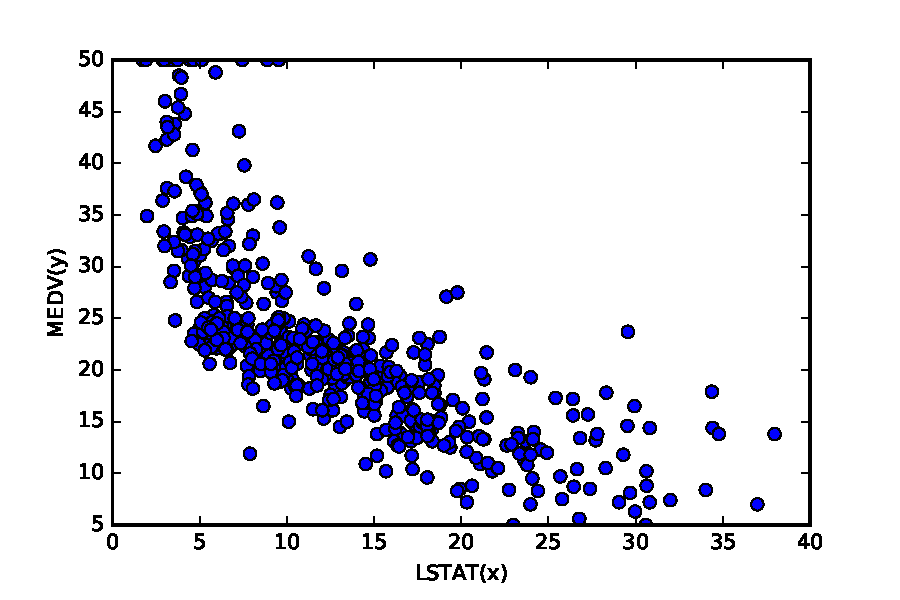
\includegraphics[scale=1]{fig1.pdf}
\end{figure}
\subsection{Problem 3.1 A1Computing the cost function J($\theta$)}
see our code 
\subsection{Problem 3.1 A2 Implmenting gradient descent}
\begin{figure}
  \caption{Fitting a linear model to the data in fig 1}
  \centering
    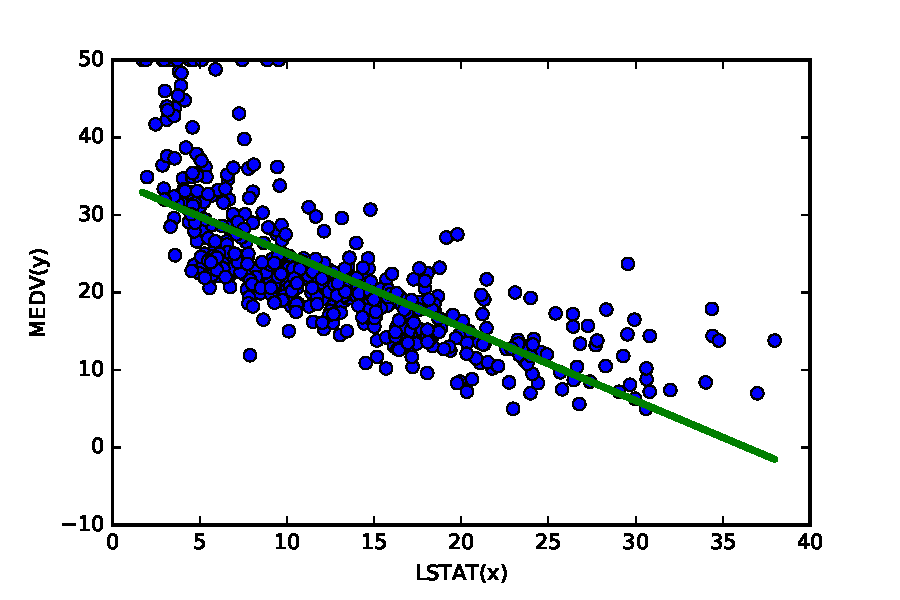
\includegraphics[scale=1]{fig2.pdf}
\end{figure}
\begin{figure}
  \caption{convergence of gradient }
  \centering
    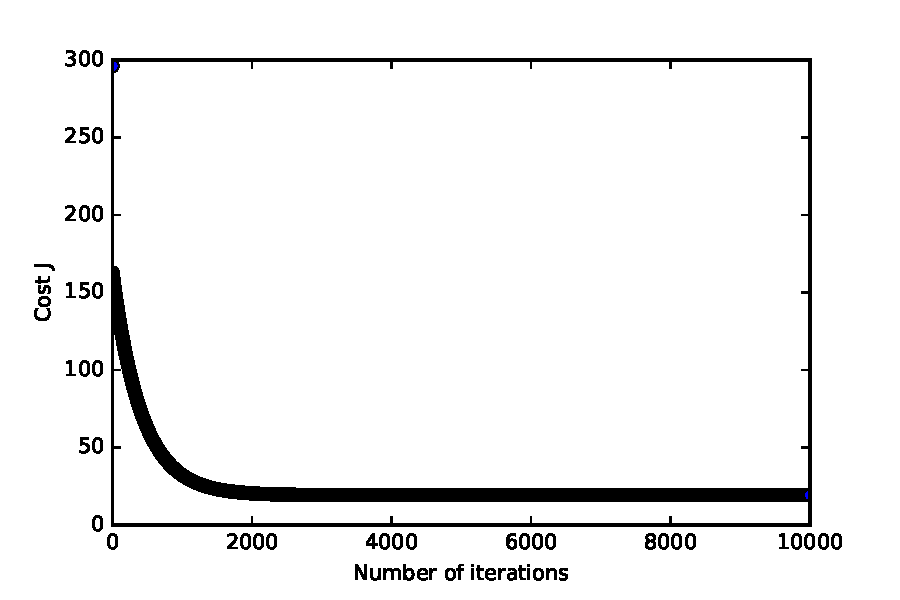
\includegraphics[scale=1]{fig4.pdf}
\end{figure}

\subsection{Problem 3.1 A3 Predicting on unseen data}
Theta found by gradient descent: [34.55363411  -0.95003694]
For lower status percentage = 5\%, we predict a median home value of 298034.494122
For lower status percentage = 50\%, we predict a median home value of -129482.128898
\begin{figure}
  \caption{Surface plot of J}
  \centering
    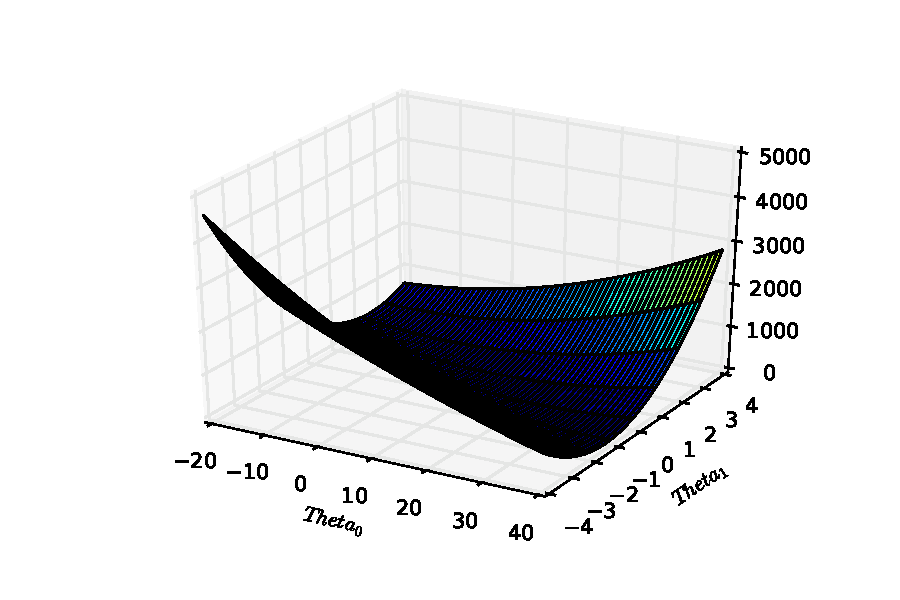
\includegraphics[scale=1]{fig3a.pdf}
\end{figure}
\begin{figure}
  \caption{contour plot of J}
  \centering
    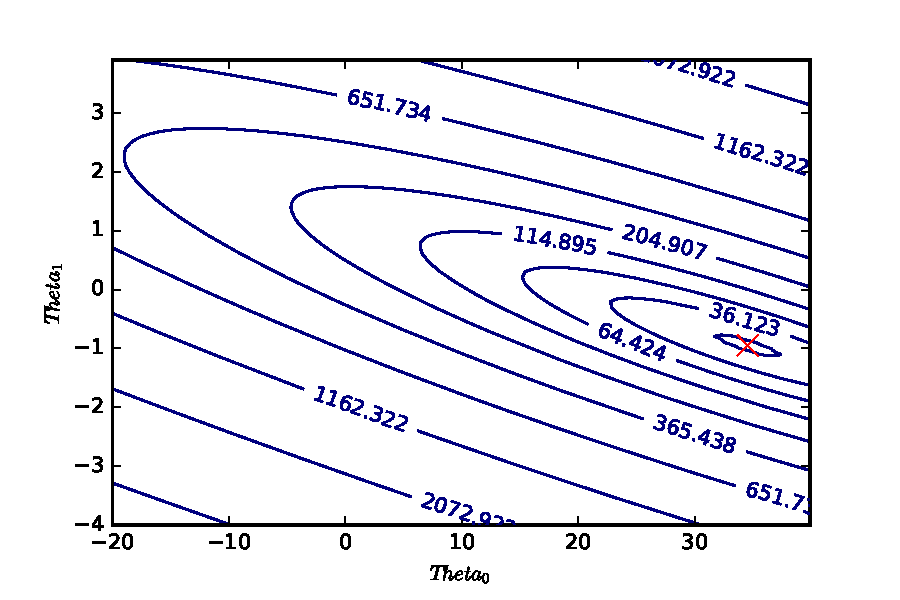
\includegraphics[scale=1]{fig3b.pdf}
\end{figure}
\subsection{assessing model quality}
The coefficients computed by sklearn:  34.5538408794  and  -0.950049353758
2  fold cross\_validation MSE =  39.5116296814
2  fold cross\_validation r\_squared =  0.510083569547

5  fold cross\_validation MSE =  42.61890333
5  fold cross\_validation r\_squared =  0.297106799977

10  fold cross\_validation MSE =  41.8292437273
10  fold cross\_validation r\_squared =  -0.18466981353
So k=2 is the best








\subsection{Problem 3.1 B Linear regression with multiple variables}
\subsection{Problem 3.1 B1Feature normalization}
see in the code
\subsection{Problem 3.1 B2 Loss function and gradient descent}
\begin{figure}
  \caption{J for multiple variables}
  \centering
    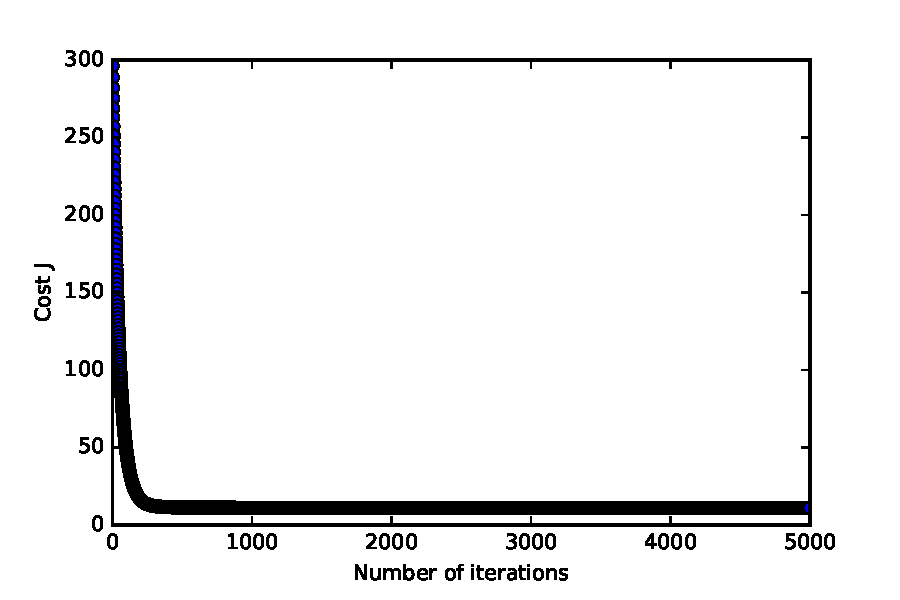
\includegraphics[scale=1]{fig5.pdf}
\end{figure}
Theta computed by gradient descent:  [  2.25328063e+01  -9.13925619e-01   1.06949712e+00   1.07531669e-01
   6.87258582e-01  -2.05340341e+00   2.67719690e+00   1.55788957e-02
  -3.10668099e+00   2.56946272e+00  -1.97453430e+00  -2.05873147e+00
   8.55982884e-01  -3.74517559e+00]

\subsection{Problem 3.1 B3 Making predictions on unseen data}

For average home in Boston suburbs, we predict a median home value of 225328.063241
The predictions match very well. Even though the theta are different but we can still have a good prediction because we have a lot of parameters. The difference of theta may come from the normalization of data.


\subsection{Problem 3.1 B4 Normal equation}

Theta computed by direct solution is:  [  3.64911033e+01  -1.07170557e-01   4.63952195e-02   2.08602395e-02
   2.68856140e+00  -1.77957587e+01   3.80475246e+00   7.51061703e-04
  -1.47575880e+00   3.05655038e-01  -1.23293463e-02  -9.53463555e-01
   9.39251272e-03  -5.25466633e-01]
For average home in Boston suburbs, we predict a median home value of 225328.063241


\subsection{Problem 3.1 B5 Convergence of gradient descent}
After running the four different learning rates provided (.01, .03, .1, and .3), we found that all converged, none with oscillation, on the same value. Thus, the best choice for a learning rate out of these four is 0.3 due to the fact that it converges the fastest and thus requires the least amount of iterations to finish training. 
\begin{figure}
  \caption{J for different learning rate}
  \centering
    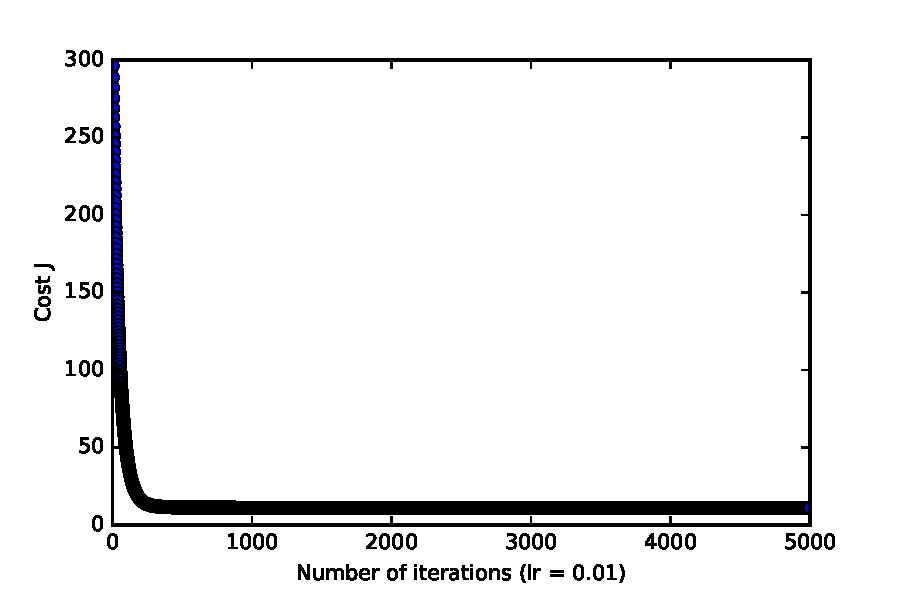
\includegraphics[scale=1]{fig001.pdf}
\end{figure}
\begin{figure}
  \caption{J for different learning rate}
  \centering
    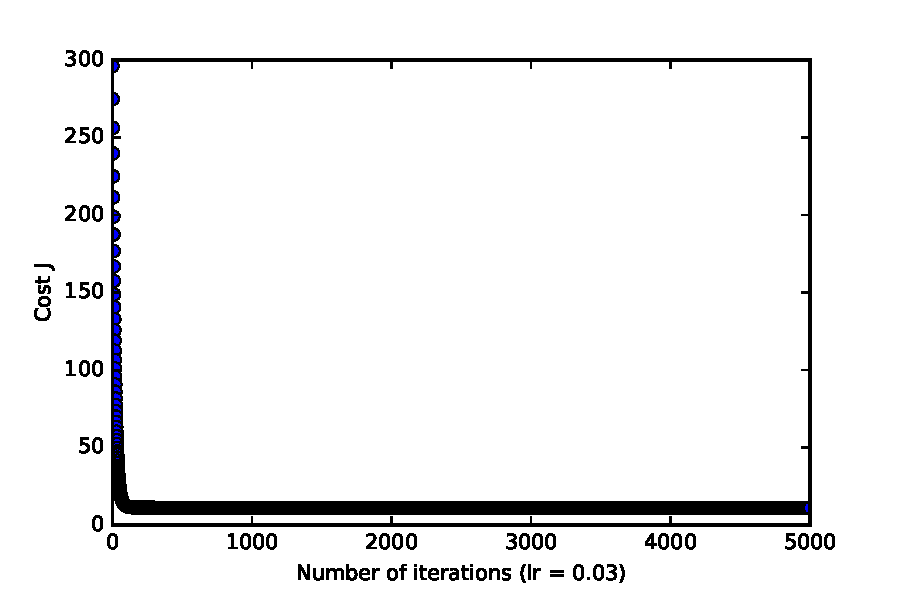
\includegraphics[scale=1]{fig003.pdf}
\end{figure}
\begin{figure}
  \caption{J for different learning rate}
  \centering
    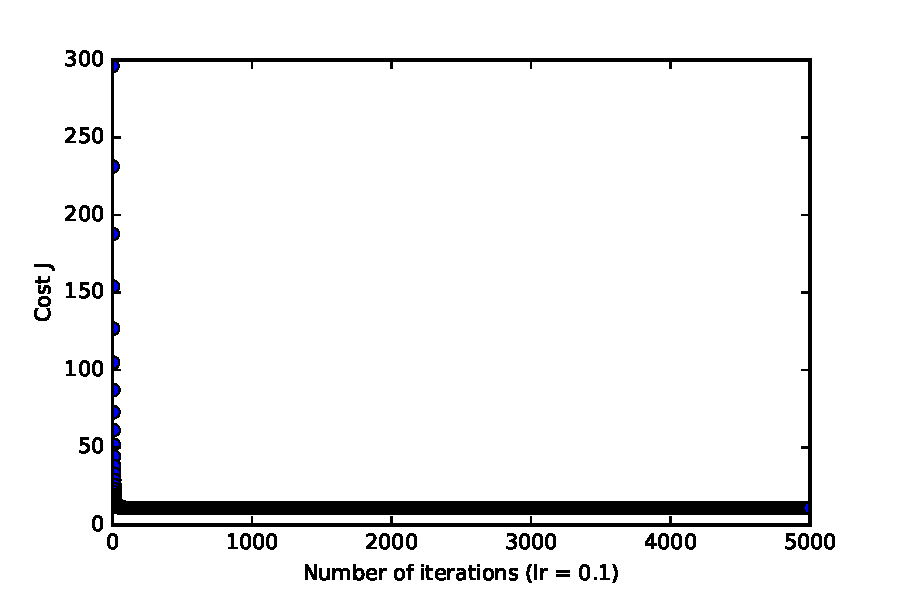
\includegraphics[scale=1]{fig01.pdf}
\end{figure}
\begin{figure}
  \caption{J for different learning rate}
  \centering
    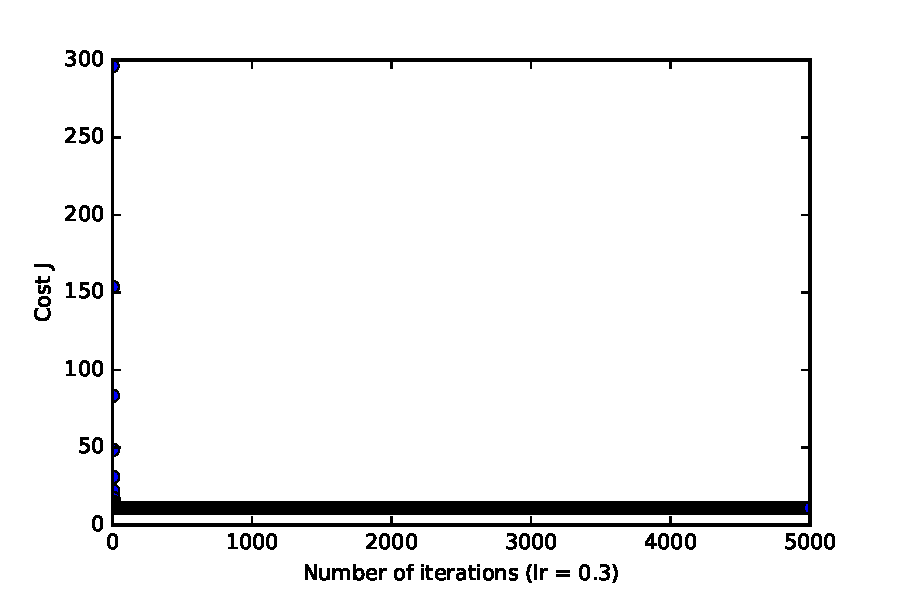
\includegraphics[scale=1]{fig03.pdf}
\end{figure}



\section{Problem 3 part 2 Implementing regularized linear regression}
\begin{figure}
  \caption{JThe training data}
  \centering
    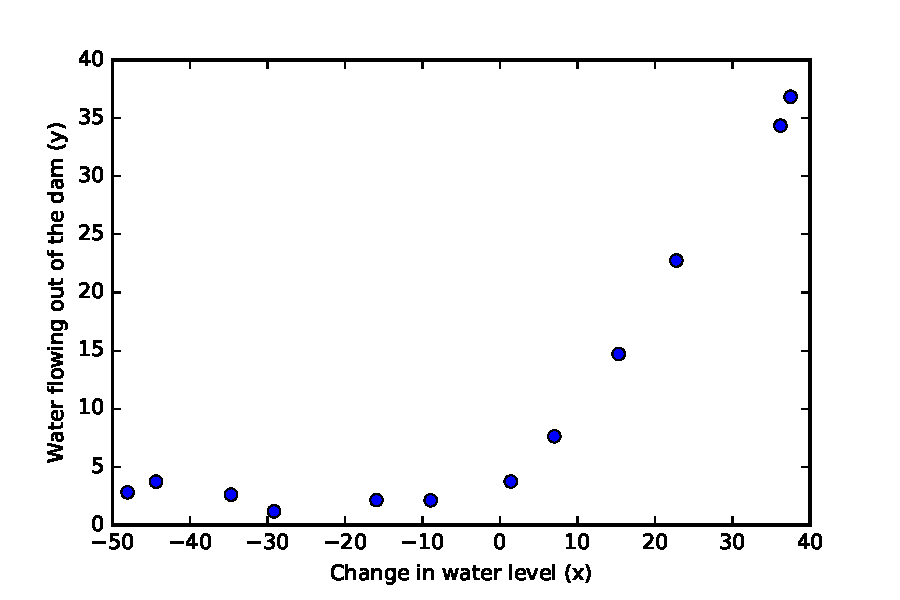
\includegraphics[scale=1]{fig6.pdf}
\end{figure}

\subsection{Problem 3.2 A1 regression cost function }
see code


\subsection{Problem 3.2 A2 Gradient of the cost function }
Learning linear regression mocel
Optimization terminated successfully.
         Current function value: 22.373906
         Iterations: 5
         Function evaluations: 6
         Gradient evaluations: 6
Theta at lambda = 0 is  [ 13.08790353   0.36777923]

\begin{figure}
  \caption{The best fit for the data}
  \centering
    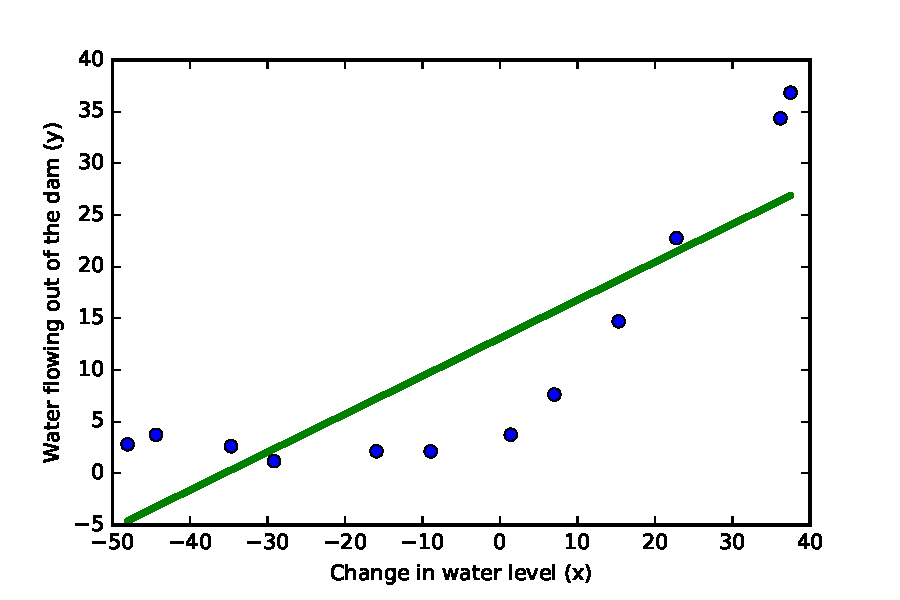
\includegraphics[scale=1]{fig7.pdf}
\end{figure}
\subsection{Problem 3.2 A3 Learning curve}

\begin{figure}
  \caption{Learning curves}
  \centering
    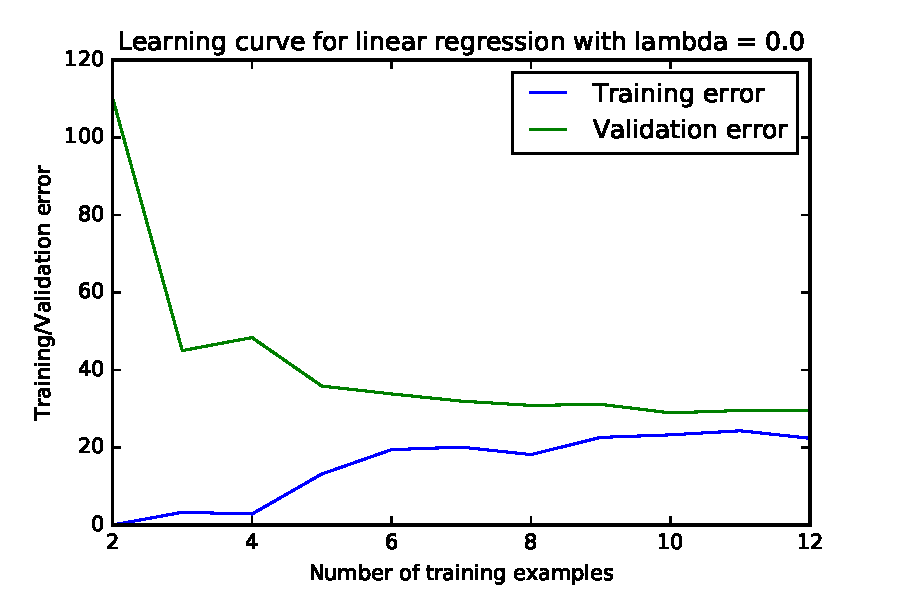
\includegraphics[scale=1]{fig8.pdf}
\end{figure}
\subsection{Learning polynomial regression models}
\begin{figure}
  \caption{Polynomial fit for reg=0 with p=6}
  \centering
    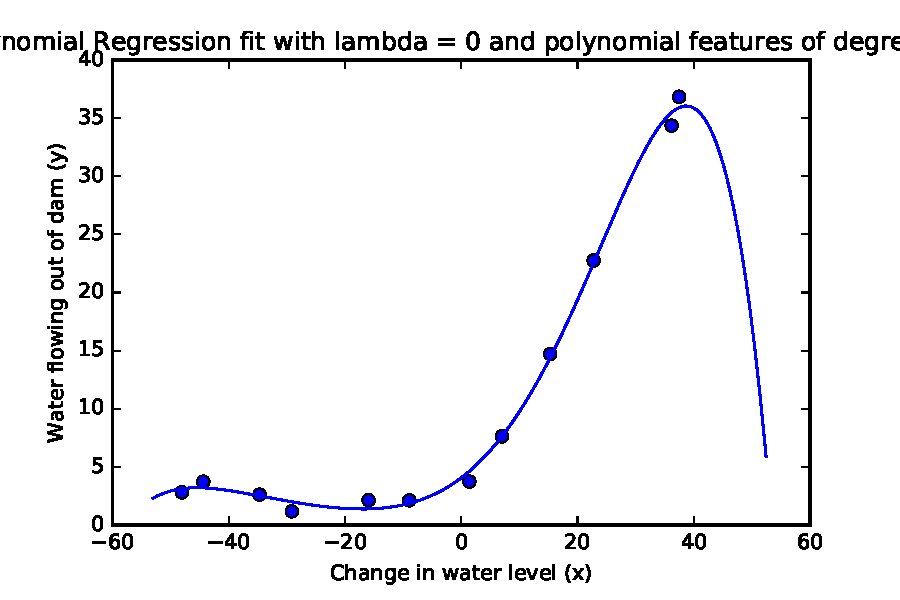
\includegraphics[scale=1]{fig9.pdf}
\end{figure}
\begin{figure}
  \caption{Learning curves for reg=0}
  \centering
    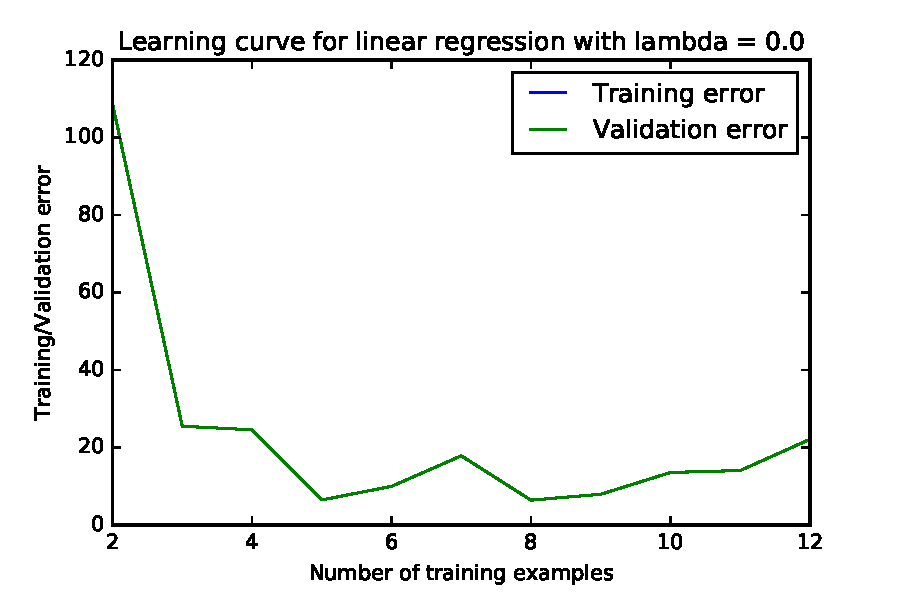
\includegraphics[scale=1]{fig10.pdf}
\end{figure}

\subsection{Problem 3.2 A4 Adjusting the regularization parameter}
We try  1,10,100
for 1:
\begin{figure}
  \caption{Polynomial fit for reg=1}
  \centering
    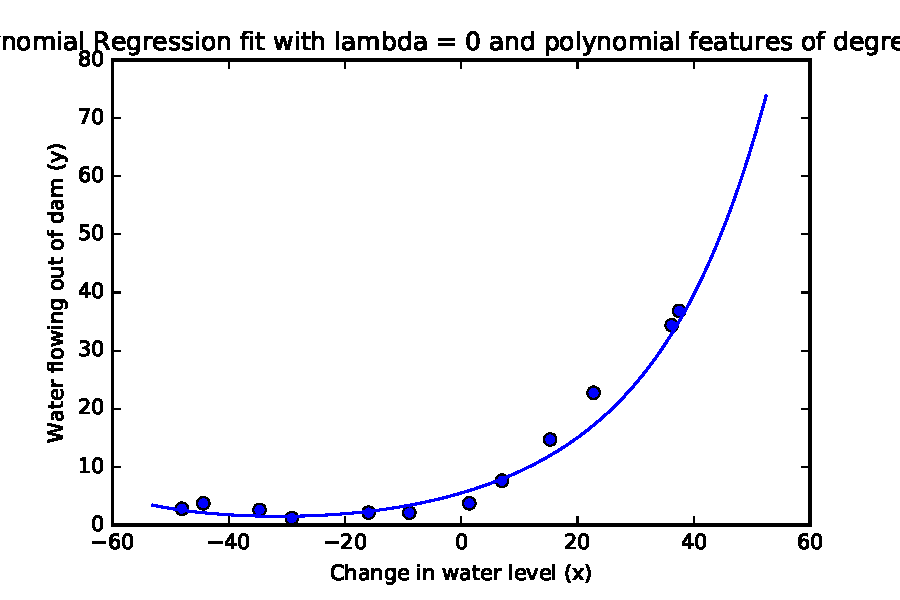
\includegraphics[scale=1]{fig91.pdf}
\end{figure}
\begin{figure}
  \caption{Learning curves for reg=1}
  \centering
    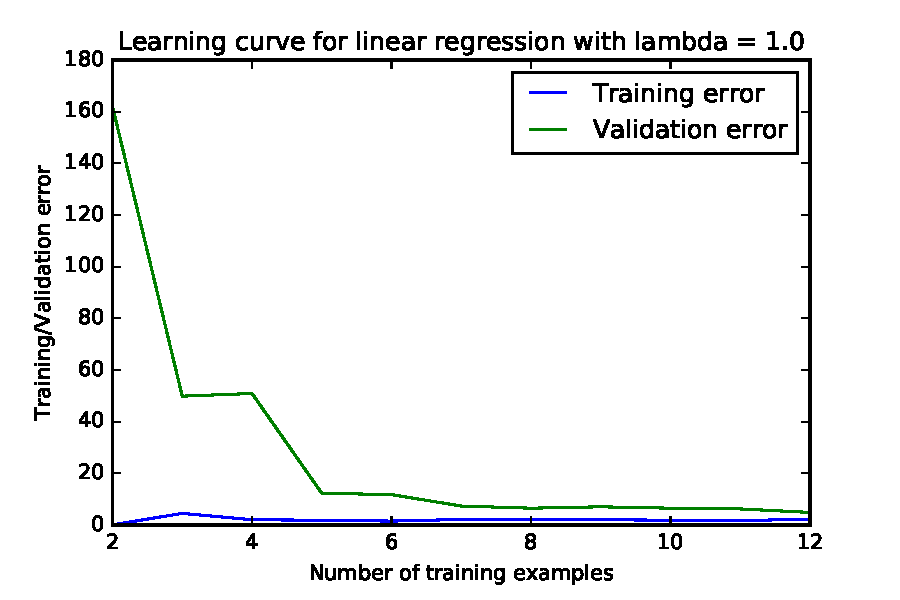
\includegraphics[scale=1]{fig101.pdf}
\end{figure}
for 10
\begin{figure}
  \caption{Polynomial fit for reg=10}
  \centering
    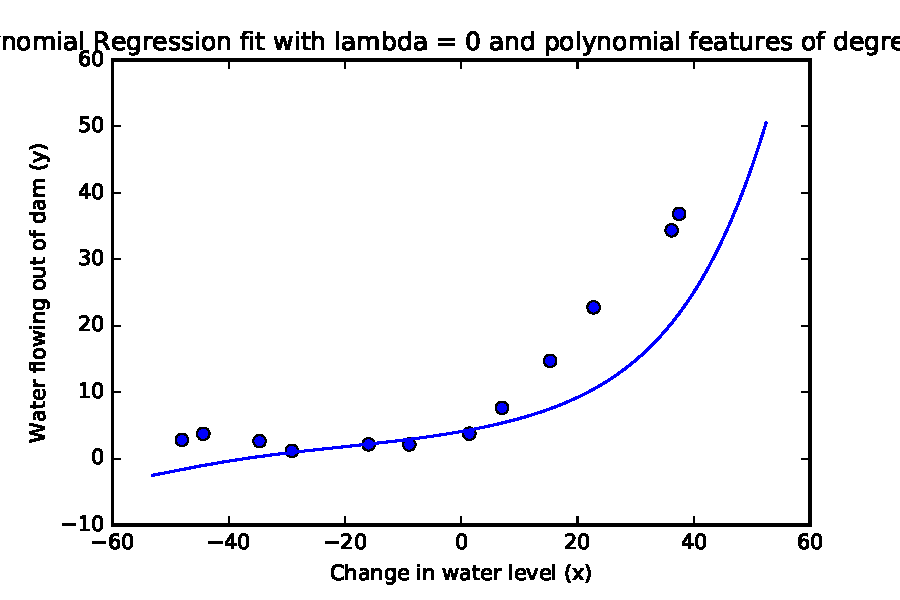
\includegraphics[scale=1]{fig910.pdf}
\end{figure}
\begin{figure}
  \caption{Learning curves for reg=10}
  \centering
    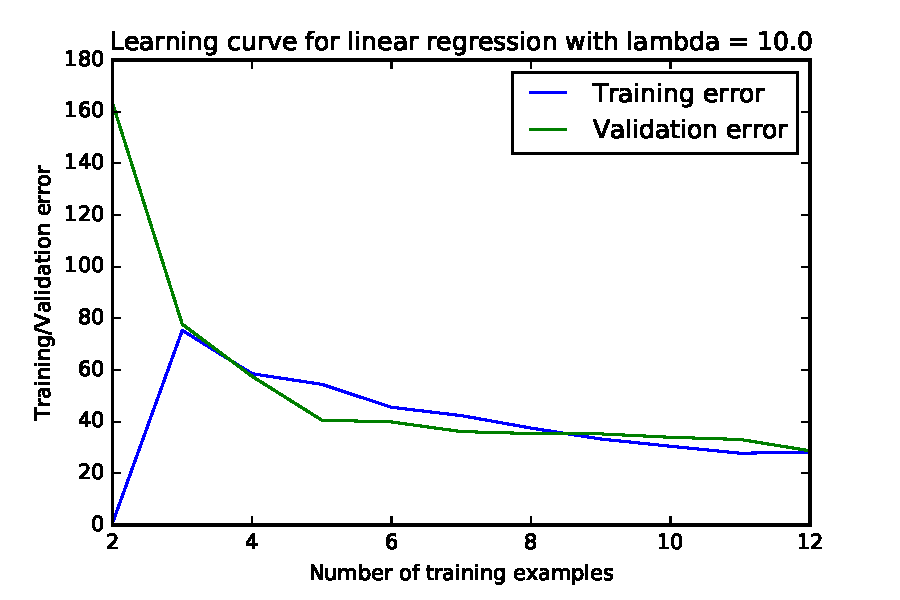
\includegraphics[scale=1]{fig1010.pdf}
\end{figure}
for 100
\begin{figure}
  \caption{Polynomial fit for reg=100}
  \centering
    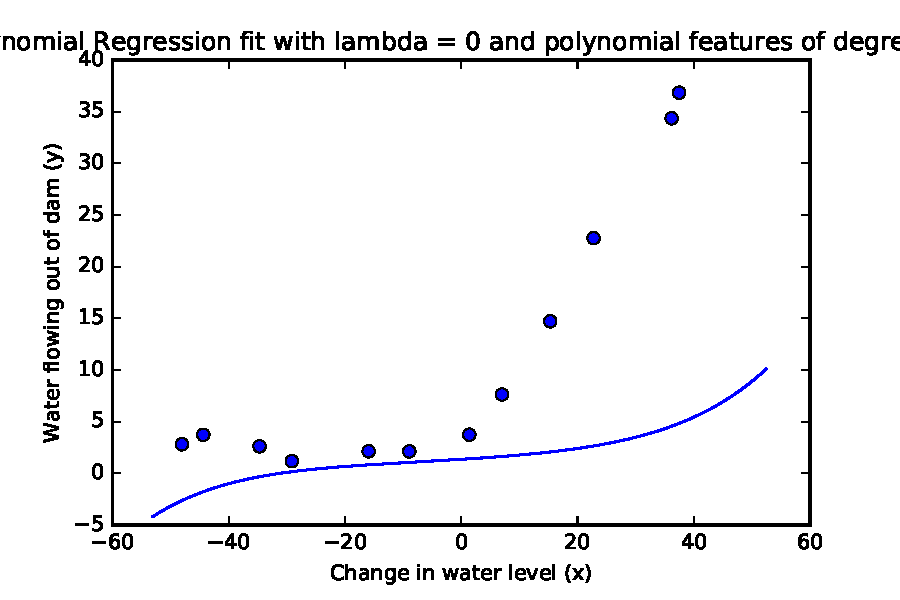
\includegraphics[scale=1]{fig9100.pdf}
\end{figure}
\begin{figure}
  \caption{Learning curves for  reg=100}
  \centering
    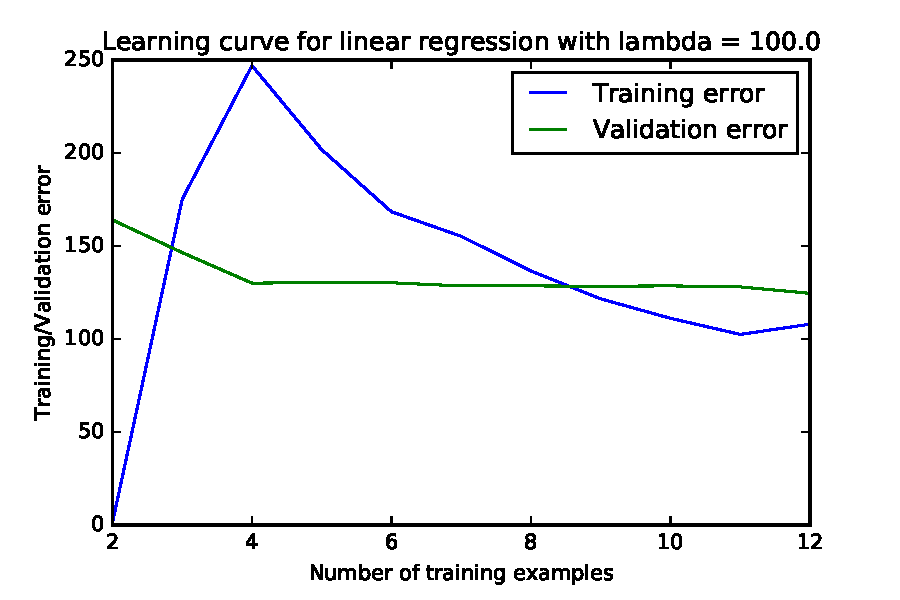
\includegraphics[scale=1]{fig10100.pdf}
\end{figure}




\subsection{Problem 3.2 A5 selecting lambda using a validation set}
Based on our error curve, We find a clear minimum for validation error between $0.3$ and $1$. As for the training data the minimum is about at $0.3$, so we make a conclusion that $0.3$ is the best choice of $\lambda$ for this problem.

\begin{figure}
  \caption{Selecting lambda}
  \centering
    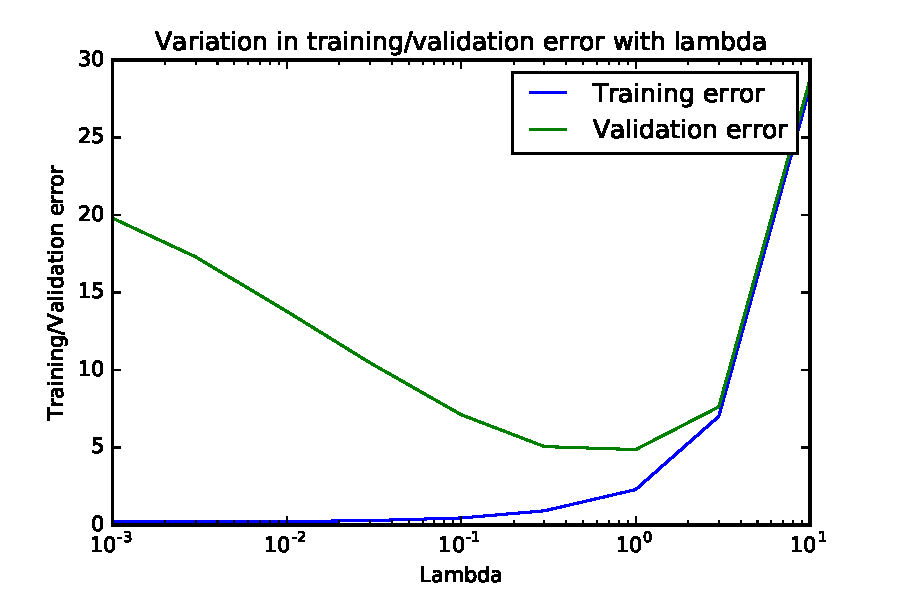
\includegraphics[scale=1]{fig12.pdf}
\end{figure}
\subsection{Problem 3.2 A6 Test error with the best model}
We find out reg=1 is the best model
\begin{figure}
  \caption{Test error with the best model}
  \centering
    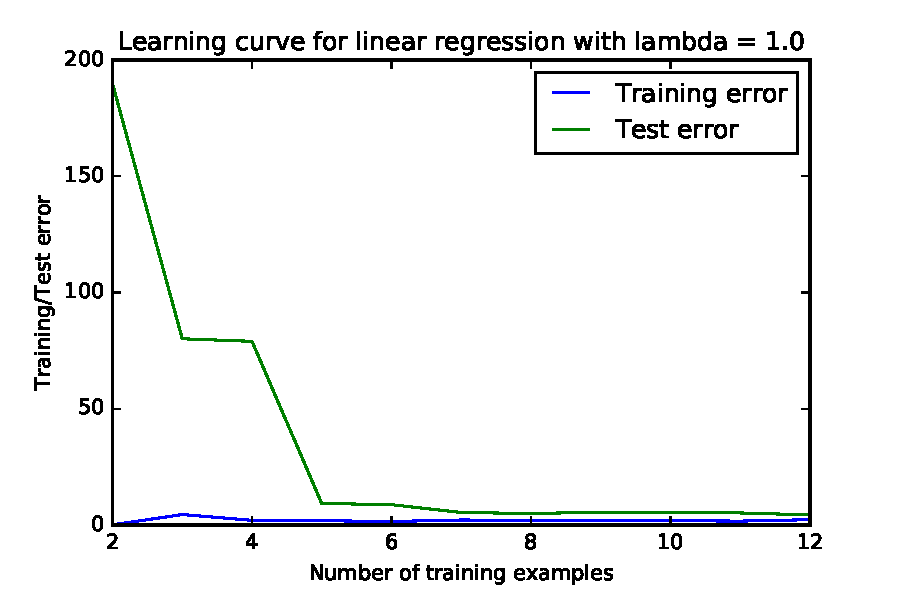
\includegraphics[scale=1]{figtest.pdf}
\end{figure}

\subsection{Problem 3.2 A6 Test error with the best model}
We plot the test error in the plot. Test error is similar to the training error
\begin{figure}
  \caption{Test error with the best model}
  \centering
    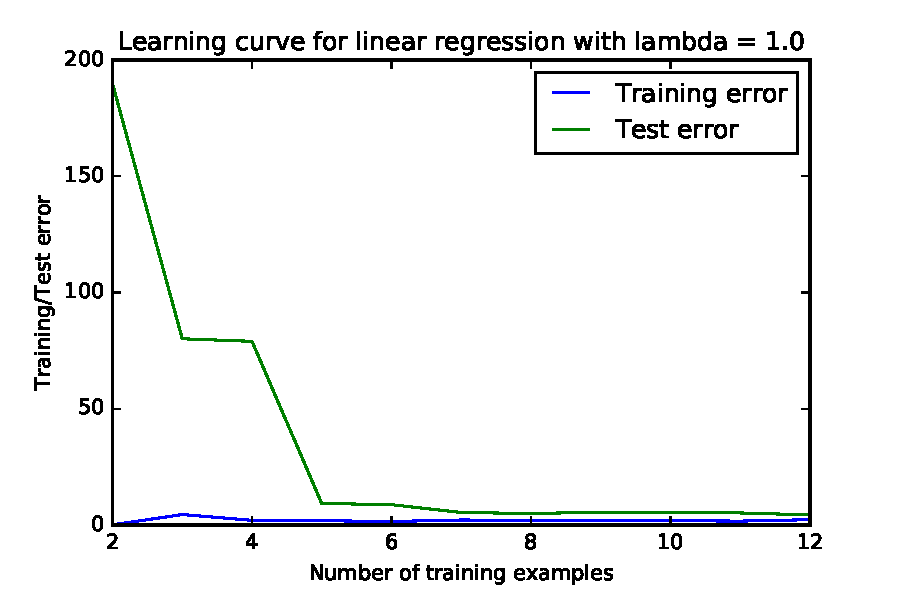
\includegraphics[scale=1]{figtest.pdf}
\end{figure}

\subsection{Problem 3.2 A7 Plotting learning curves with randomly examples}

\begin{figure}
  \caption{Averaged Learning curve for lambda=1}
  \centering
    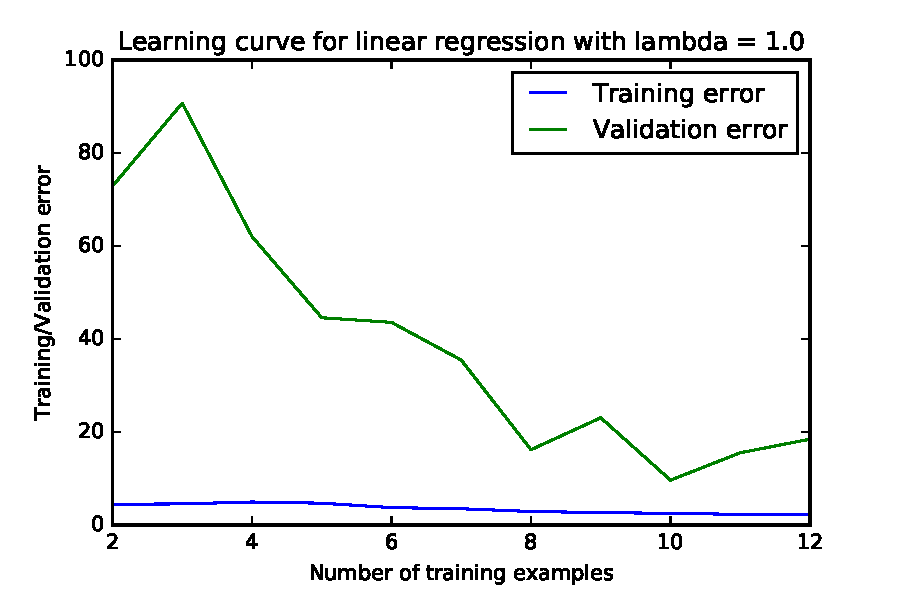
\includegraphics[scale=1]{fig11.pdf}
\end{figure}

\end{document}